\documentclass[12pt, a4paper]{article}

% Packages and Formatting
\usepackage{../../sub/mystyle_general}
\usepackage{../../sub/mystyle_article}


\title{Lista 8 - Introdução a Análise de Dados \\
	Análise de Dados \\
	Gabarito}
\author{Guilherme Masuko}
\date{May 2023}
%\affil{}



\definecolor{dkgreen}{rgb}{0,0.6,0}
\definecolor{gray}{rgb}{0.5,0.5,0.5}
\definecolor{mauve}{rgb}{0.58,0,0.82}

\lstset{frame=tb,
	language=R,
	aboveskip=3mm,
	belowskip=3mm,
	showstringspaces=false,
	columns=flexible,
	basicstyle={\small\ttfamily},
	numbers=none,
	numberstyle=\tiny\color{gray},
	keywordstyle=\color{blue},
	commentstyle=\color{dkgreen},
	stringstyle=\color{mauve},
	breaklines=true,
	breakatwhitespace=true,
	tabsize=3
}

\lstset{inputencoding=utf8/latin1}


\begin{document}

% Title Page
\clearpage
\maketitle
\thispagestyle{empty}

Para essa lista vamos analisar a população (total e urbana) de alguns países. Utilizaremos os dados do banco mundial para isso. Essa base de dados está vinculada ao R através do pacote \texttt{WDI}\footnote{\url{https://www.r-project.org/nosvn/pandoc/WDI.html}}.

Para acessar os dados, precisamos instalar e chamar o pacote. Os dados que queremos estão armazenados pelo \texttt{indicador = c("total\_pop"="SP.POP.TOTL", "urban\_pop"="SP.URB.TOTL")}. O parâmetro \texttt{country} recebe as siglas dos países que estamos interessados em analisar o PIB per capita. \texttt{start} e \texttt{end} referenciam o intervalo temporal dos dados. A seguir o script.

\lstinputlisting[language=R]{codes/intro.R}



\textbf{Questão 1}

Crie as seguintes colunas:

\begin{itemize}
	\item[\textbf{a)}] Taxa de população urbana.
	
	
	\textbf{Solução}
	
	\lstinputlisting[language=R]{codes/solution1a.R}
	
	
	
	\item[\textbf{b)}] Taxa de crescimento da população (total e urbana).
	
	
	\textbf{Solução}

	\lstinputlisting[language=R]{codes/solution1b.R}
	
	
	
\end{itemize}



\textbf{Questão 2}

Crie uma coluna contendo a região (continente) de cada país (crie utilizando código, sem utilizar o parâmetro \texttt{extra = TRUE}).


\textbf{Solução}

\lstinputlisting[language=R]{codes/solution2.R}



\textbf{Questão 3}

Calcule as estatísticas média, mínimo e máximo para as seguintes variáveis.

\begin{itemize}
	\item[\textbf{a)}] Taxa de população urbana agrupados por região para o ano de 2020.
	
	
	\textbf{Solução}
	
	\lstinputlisting[language=R]{codes/solution3a.R}
	
	
	
	\item[\textbf{b)}] Taxa de crescimento da população total agrupados por região para o ano de 2010.
	
	
	\textbf{Solução}
	
	\lstinputlisting[language=R]{codes/solution3b.R}
	
	
	
	\item[\textbf{c)}] Taxa de crescimento da população urbana agrupados por região para o ano de 2016.
	
	
	\textbf{Solução}
	
	\lstinputlisting[language=R]{codes/solution3c.R}
	
	
	
\end{itemize}



\textbf{Questão 4}

Calcule a média, mínimo e máximo da taxa de população urbana, taxa de crescimento da população total e taxa de crescimento da população urbana, para cada país durante todo o período que temos na amostra.



\textbf{Solução}

\lstinputlisting[language=R]{codes/solution4.R}



\textbf{Questão 5}

Calcule as médias de cada uma das variáveis abaixo agrupados por país (o resultado será uma média para cada país, assim como na questão anterior). A partir desse resultado, calcule o máximo e o mínimo dessas médias agrupados por região.

\begin{itemize}
	\item[\textbf{a)}] Taxa de população urbana.
	
	
	\textbf{Solução}
	
	\lstinputlisting[language=R]{codes/solution5a.R}
	
	
	
	\item[\textbf{b)}] Taxa de crescimento da população total.
	
	
	\textbf{Solução}
	
	\lstinputlisting[language=R]{codes/solution5b.R}
	
	
	
	\item[\textbf{c)}] Taxa de crescimento da população urbana.
	
	
	\textbf{Solução}
	
	\lstinputlisting[language=R]{codes/solution5c.R}
	
	
	
\end{itemize}



\textbf{Questão 6}

Crie um \texttt{data.frame} para cada país (cada um com o nome do país, tudo em lower case), contendo apenas as colunas \texttt{country}, \texttt{year} e a coluna contendo as informações sobre a taxa de população urbana.



\textbf{Solução}

\lstinputlisting[language=R]{codes/solution6.R}



\textbf{Questão 7}

Crie uma função que recebe um dataframe como parâmetro. Essa função deve fazer as seguintes manipulações nesse dataframe:

\begin{itemize}
	\item Renomear a coluna contendo as informações sobre a taxa de população urbana para o nome do país do respectivo dataframe.
	\item Manter somente as colunas \texttt{year} e a (agora) do nome do país.
\end{itemize}

Use a função para alterar todos os dataframes dos países.



\textbf{Solução}

\lstinputlisting[language=R]{codes/solution7.R}



\textbf{Questão 8}

Una todos dataframes. Renomeie as colunas dos países com nomes compostos, alterando o espaço entre os nomes por um underline "\_". 

Faça um gráfico apresentando a série temporal da taxa de população urbana para cada país, um para cada região.


\textbf{Solução}

\lstinputlisting[language=R]{codes/solution8.R}



\begin{itemize}
	\item[\textbf{a)}] América Latina.
	
	
	\textbf{Solução}
	
	\lstinputlisting[language=R]{codes/solution8a.R}
	
	
	\begin{figure}[H]
		\caption{América Latina}
		\centering
		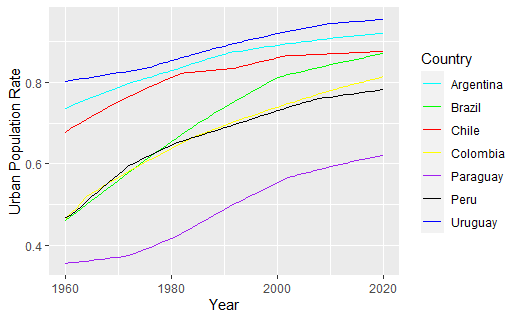
\includegraphics[scale=1.2]{images/latin_america.png}
	\end{figure}
	
	
	
	\item[\textbf{b)}] América do Norte.
	
	
	\textbf{Solução}
	
	\lstinputlisting[language=R]{codes/solution8b.R}
	
	
	\begin{figure}[H]
		\caption{América do Norte}
		\centering
		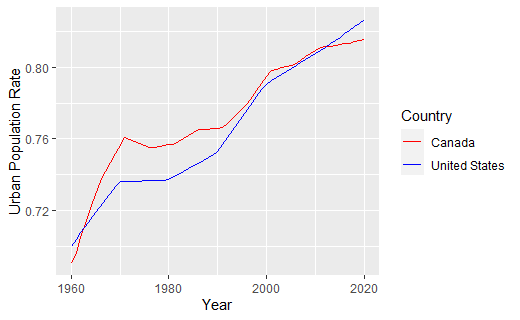
\includegraphics[scale=1.2]{images/north_america.png}
	\end{figure}
	
	
	
	\item[\textbf{c)}] Europa.
	
	
	\textbf{Solução}
	
	\lstinputlisting[language=R]{codes/solution8c.R}
	
	
	\begin{figure}[H]
		\caption{Europa}
		\centering
		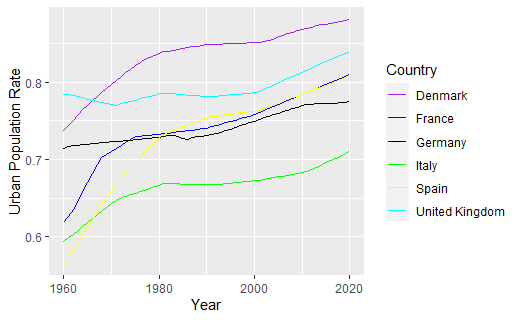
\includegraphics[scale=1.2]{images/europe.png}
	\end{figure}
	
	
	
\end{itemize}


	
\end{document}